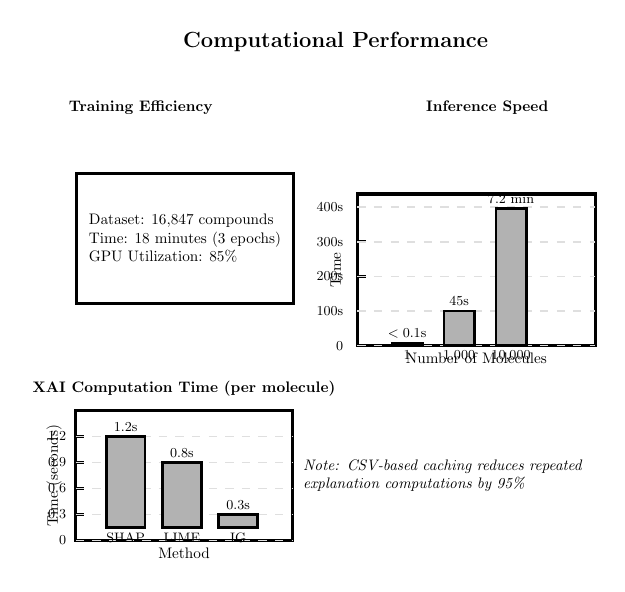
\begin{tikzpicture}[font=\normalsize, scale=0.55, transform shape]

% Title - large and clear
\node[font=\bfseries\Large] at (6,13.5) {Computational Performance};

% ========== Section 1: Training Efficiency ==========
% Positioned top-left with clear spacing
\node[font=\bfseries\normalsize] at (1.5,12) {Training Efficiency};
\node[draw, rectangle, minimum width=5cm, minimum height=3cm, align=left, anchor=north west, line width=1.2pt, fill=white] (training) at (0,10.5) {
Dataset: 16,847 compounds\\
Time: 18 minutes (3 epochs)\\
GPU Utilization: 85\%
};

% ========== Section 2: Inference Speed ==========
% Positioned top-right with clear spacing
\node[font=\bfseries\normalsize] at (9.5,12) {Inference Speed};

% Inference Speed Chart - larger and clearer
% Background box
\draw[thick, line width=1.2pt] (6.5,6.5) rectangle (12,10);

% Y-axis label - larger font
\node[rotate=90, font=\normalsize] at (6,8.25) {Time};

% X-axis label - larger font
\node[font=\normalsize] at (9.25,6.2) {Number of Molecules};

% Y-axis ticks and grid lines - clearer
\foreach \y/\label in {6.5/0, 7.3/100s, 8.1/200s, 8.9/300s, 9.7/400s} {
    \draw[thick, line width=1pt] (6.5,\y) -- (6.7,\y);
    \node[left, font=\small] at (6.3,\y) {\label};
    \draw[gray!25, line width=0.6pt, dashed] (6.5,\y) -- (12,\y);
}

% Bar 1: 1 molecule (<0.1s) - clearer positioning
\filldraw[fill=gray!60, draw=black, thick, line width=1pt] (7.3,6.5) rectangle (8,6.55);
\node[above, font=\small] at (7.65,6.55) {$<0.1$s};
\node[below, font=\small] at (7.65,6.5) {1};

% Bar 2: 1,000 molecules (45s) - clearer positioning
\filldraw[fill=gray!60, draw=black, thick, line width=1pt] (8.5,6.5) rectangle (9.2,7.3);
\node[above, font=\small] at (8.85,7.3) {45s};
\node[below, font=\small] at (8.85,6.5) {1,000};

% Bar 3: 10,000 molecules (7.2 min = 432s) - clearer positioning
\filldraw[fill=gray!60, draw=black, thick, line width=1pt] (9.7,6.5) rectangle (10.4,9.66);
\node[above, font=\small] at (10.05,9.66) {7.2 min};
\node[below, font=\small] at (10.05,6.5) {10,000};

% ========== Section 3: XAI Computation Time ==========
% Positioned bottom-left with clear separation
\node[font=\bfseries\normalsize] at (2.5,5.5) {XAI Computation Time (per molecule)};

% XAI Chart - larger and clearer
% Background box
\draw[thick, line width=1.2pt] (0,2) rectangle (5,5);

% Y-axis label - larger font
\node[rotate=90, font=\normalsize] at (-0.5,3.5) {Time (seconds)};

% X-axis label - larger font
\node[font=\normalsize] at (2.5,1.7) {Method};

% Y-axis ticks and grid lines - clearer
\foreach \y/\label in {2/0, 2.6/0.3, 3.2/0.6, 3.8/0.9, 4.4/1.2} {
    \draw[thick, line width=1pt] (0,\y) -- (0.2,\y);
    \node[left, font=\small] at (-0.1,\y) {\label};
    \draw[gray!25, line width=0.6pt, dashed] (0,\y) -- (5,\y);
}

% Bar 1: SHAP (1.2s) - clearer bars
\filldraw[fill=gray!60, draw=black, thick, line width=1pt] (0.7,2.3) rectangle (1.6,4.4);
\node[above, font=\small] at (1.15,4.4) {1.2s};
\node[below, font=\small] at (1.15,2.3) {SHAP};

% Bar 2: LIME (0.8s) - clearer bars
\filldraw[fill=gray!60, draw=black, thick, line width=1pt] (2,2.3) rectangle (2.9,3.8);
\node[above, font=\small] at (2.45,3.8) {0.8s};
\node[below, font=\small] at (2.45,2.3) {LIME};

% Bar 3: Integrated Gradients (0.3s) - clearer bars
\filldraw[fill=gray!60, draw=black, thick, line width=1pt] (3.3,2.3) rectangle (4.2,2.6);
\node[above, font=\small] at (3.75,2.6) {0.3s};
\node[below, font=\small] at (3.75,2.3) {IG};

% Note - positioned bottom-right with clear separation and larger font
\node[font=\itshape\normalsize, align=left, text width=6.5cm] at (8.5,3.5) {
Note: CSV-based caching reduces repeated explanation computations by 95\%
};

\end{tikzpicture}
